% ------------------------------------------
%  MASTER THESIS DISSERTATION
% ------------------------------------------
% Author:
%
% Advisors:
%
% ------------------------------------------
\documentclass[11pt,twoside,openright,a4paper]{report}
\usepackage[utf8]{inputenc}

% Set document margins to 1in in all sides
\usepackage[margin=2.5cm]{geometry}
% Line spacing package
\usepackage{graphicx, helvet, hyperref, setspace}
\usepackage{wrapfig}
\usepackage{subfig}
\usepackage[portuguese,english]{babel}
\usepackage[acronym, toc]{glossaries}
% Extra stuff file
% This file is included before begin{document} environment
% Use this to include extra packages and define your own commands
% This way, you can easily grab a most recent version
% of dissertation.tex file from the original repo

% Built the glossary when the main file is built.
\makeglossaries
% Set main font to Arial
\renewcommand{\familydefault}{\sfdefault}
% Define keywords macro
\providecommand{\keywords}[1]{\textbf{Keywords:} #1}
% Define the NewPage macro
\newcommand*\NewPage{\newpage\null\thispagestyle{empty}\cleardoublepage}
% Abstract-en page numbering
\newcommand {\abstractEnglishPageNumber} {\thispagestyle{plain}\setcounter{page}{\abstractEnglishPage}}
% Abstract-pt page numbering
\newcommand {\abstractPortuguesePageNumber} {\thispagestyle{plain}\setcounter{page}{\abstractPortuguesePage}}
% Section numbering depth
\setcounter{secnumdepth}{2}
% Table of contents depth
\setcounter{tocdepth}{3}
% Set line spacing to 1.5cm
\onehalfspacing
% Page numbering
\pagestyle{plain}

% Glossary-File
% Glossary Definition

\newglossaryentry{MSc}{name={MSc}, description={Masters degree in the area of Science.}}

% Acronym-File
% Acronym Definition

\newacronym{IST}{IST}{Instituto Superior T\'ecnico}
\newacronym{ISR}{ISR}{Institute for Systems and Robotics}
\newacronym{Mbot}{Mbot}{Monarch Robot}
\newacronym{DoF}{DoF}{Degrees Of Freedom}
\newacronym{IBVS}{IBVS}{Image Based Visual Servoing}
\newacronym{PBVS}{PBVS}{Pose Based Visual Servoing}
\newacronym{YOLO}{YOLO}{You Only Look Once}
\newacronym{VS}{VS}{Visual Servoing}
\newacronym{ROS}{ROS}{Robot Operating System}
\newacronym{ViSP}{ViSP}{Visual Servoing Platform}
\newacronym{URDF}{URDF}{Unified Robot description Format}
\newacronym{COG}{COG}{Center Of Gravity}



% ------------------------------------------
% MASTER THESIS DISSERTATION
% ------------------------------------------

\begin{document}
\pagenumbering{gobble}% Remove page numbers (and reset to 1)
\clearpage
\thispagestyle{empty}
%!TEX root = ./dissertation.tex

% Dissertation basic information
\newcommand {\Title} {Internship Report}
\newcommand {\Subtitle} {Applying an Image Based Visual Servoing control law to Mbot 7\gls{DoF} with an EYE-IN-HAND configuration}
\newcommand {\StudentName} {CHOPOT Louis}
\newcommand {\DegreeName} {Master in Robotics}
\newcommand {\Supervisors} {{\large Prof. Pedro Lima}}

% Include or not include acknowledgments
\def \includeAcknowledgments{1}

% Include or not include glossary
\def \includeGlossary{0}

% Date
\newcommand {\Month} {March-September}
\newcommand {\Year} {2018}

% Acknowledgments page number
\def \acknowledgmentsPage{1}

% Abstract-en page numbering
\def \abstractEnglishPage{3}

% You can define your own variables here

%!TEX root = ./dissertation.tex

% ---------------------------------------------------------
%   MASTER THESIS DISSERTATION COVER
% ---------------------------------------------------------
\begin{titlepage}
% ---------------------------------------------------------
%  INSTITUTION LOGO
% ---------------------------------------------------------
\begin{figure}[!h]
\centering

\includegraphics[width=0.55\linewidth]{images/ist_logo}

\includegraphics[width=0.42\linewidth]{images/download.png}\\[1.50cm]
\end{figure}

\begin{center}
% ---------------------------------------------------------
%  MASTER THESIS DISSERTATION TITLE
% ---------------------------------------------------------
{\LARGE \textbf{\Title}}\\[1.0cm]
% ---------------------------------------------------------
%  MASTER THESIS DISSERTATION SUBTITLE
% ---------------------------------------------------------
{\Large \Subtitle}\\[4.0cm]
% ---------------------------------------------------------
%  AUTHOR NAME (FULL)
% ---------------------------------------------------------
{\Large \textbf{\StudentName}}\\[1.0cm]
% -----------------------------------------------------------------
%  COURSE NAME
% -----------------------------------------------------------------
{\LARGE \textbf{\DegreeName}}\\[3.0cm]

% -----------------------------------------------------------------
%  ADVISORS NAME
% ---------------------------------------------------------
\begin{minipage}[t]{.5\textwidth}
  \begin{flushright}
    {\large Advisor(s)/Supervisor(s):\:}
  \end{flushright}
\end{minipage}%
\begin{minipage}[t]{.5\textwidth}
  \begin{flushleft}
    {\Supervisors}
  \end{flushleft}
\end{minipage}\\[5.0cm]

% ---------------------------------------------------------
%  DATE (MONTH AND YEAR)
% ---------------------------------------------------------
{\Large \textbf{\Month\:\Year}}\\
\end{center}
\end{titlepage}
\NewPage

\pagenumbering{roman}

% Table of contents
\tableofcontents
% A new page is necessary only if table of contents has an even number of pages

% List of figures
\addcontentsline{toc}{chapter}{\listfigurename}
\listoffigures

% List of acronyms
\printglossary[type=\acronymtype]

\pagenumbering{arabic}% Arabic page numbers (and reset to 1)

%!TEX root = ../dissertation.tex

% Entry point for chapters
% In this file you define the order
% in which the chapters are included

% Chapters
%!TEX root = ../dissertation.tex

\chapter{Introduction}
\label{chapter:introduction}
\section{Context and environment of the internship}

During my first semester of my international year, I have been doing a research internship in \gls{IST} in Lisbon, Portugal. This internship took place in \gls{ISR} which is part of \gls{IST}.

During this period I have been part of a robotic research team called SocRob that stands for Social Robotic (before it was for Soccer Robot). This team has a long history in robotic competitions, specially European Robotic League and RoboCup. I had the chance to participate to both of these competitions during my internship. SocRob was at the origin participating to these competitions with soccer robot: robots playing soccer against another robot team with the goal to score more points than the other team. After a few years, it was decided to participate in the same competitions but in an other league called: robot for home. Soccer robots were abandoned to a new robot called \gls{Mbot}.

\gls{Mbot}, is a robot designed at the origin to provide company and interaction to kids that have difficulties to have social interaction with humans (\ref{Mbot}). He was able to communicate through his screen and his face was showing emotions through the led systems on his "face" (eyes and mouth). He was able to play various game and activities with kids. The design was made by a company called IDMind. Six \glspl{Mbot} are still in activity in hospitals of the Lisbon area. The Monarch project reaching an end, Researchers working in \gls{ISR} decided to upgrade two \glspl{Mbot} to be able to participate to the home robotic league. \\[0.05cm]

\begin{figure} [!h]
    \centering
    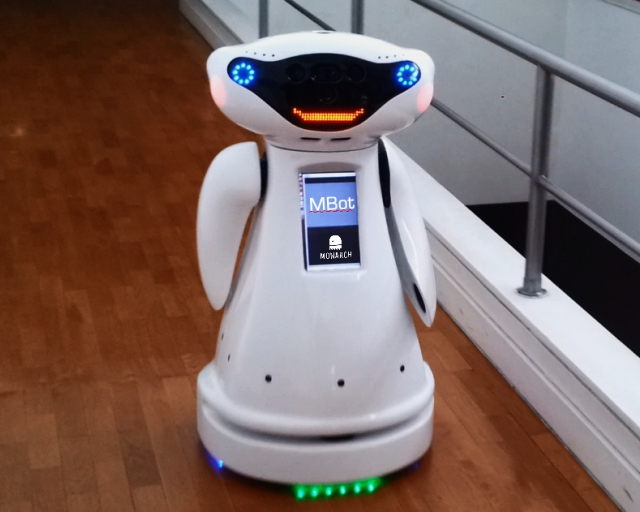
\includegraphics[width=0.30\linewidth]{images/MBOT_01s.jpg}
    \caption{Mbot, as it was designed for Monarch Project}
    \label{Mbot}
\end{figure}
\newpage

Mbot was upgraded by the SocRob@Home team \ref{Mbot_upgraded} in \gls{ISR}. It was added a robotic arm (a Cython Gamma 1500) that has 7 \gls{DoF}. It was also upgraded in many others aspects, like adding an RGB-D camera on the head, having some speakers and a microphone to be able to speak and to understand people talking to him. Also, these hardware modifications have lead to software upgrade. Multiple research topics are experimented on Mbot in \gls{ISR}, for example : Natural Language Understanding, SLAM and navigation, people recognition and following. It's an awesome platform of field testing for researchers that is improving every year and that is being tested in robotic competitions. \\[0.05cm]

\begin{figure} [!h]
    \centering
    \includegraphics[width=0.35\linewidth]{images/IMG_20180908_165314.jpg}
    \caption{Mbot, upgraded by the SocRob@Home team}
    \label{Mbot_upgraded}
\end{figure}


My internship took place in this context of research and improvement on Mbot with the goal to test these improvements in robotic competitions. SocRob@Home team is composed by various type of researchers and students, there are some PhD students, some Master students and also some research engineers. During the time I was part of this team, the number of people varied from 5 to 15 peoples working on the robot. It is a relative big team for a university project and inside ISR, SocRob@Home was the biggest robotic team. Inside the SocRob@Home team, I was part of the manipulation team, that was composed by 3 or 4 people. This team is focused on interaction and manipulation of object with the arm of Mbot. I had the chance to participate with this team to RoboCup 2018 that took place in Montreal, Canada and a challenge of the European Robotic League, that took place in Madrid, Spain.\\[0.1cm]

The laboratory where my internship took place is at the 8th floor of the North tower in IST campus in Alameda \ref{IST}. It's the historical campus of IST. It's situated in the center of Lisbon. IST is one of the oldest university of Portugal and has also the status of engineering school that is unique in Portugal. It was founded in 1911 and it's the largest (6000 graduated students per year) and most prestigious engineering school of Portugal. \\[0.3cm]

\begin{figure} [!ht]
    \centering
    \includegraphics[width=1\linewidth]{images/panoramaIST.png}
    \caption{IST campus, on the right the North tower, Lisbon}
    \label{IST}
\end{figure}

The laboratory where I worked most of the time was very different from what I knew. It was a large area with multiple teams working at the time: one team working on a robot to assist fireman, on team on sub aquatic robotic and one team working on drones. For our team and to be able to work on a home environments, an entire flat was rebuild inside the laboratory with a kitchen, a bathroom, a room and a living room \ref{laboratory}. In this flat, robotic competitions are organized and It was a nice area to train the robot to work in a realistic home environment.\\[0.05cm]

\begin{figure} [!ht]
    \centering
    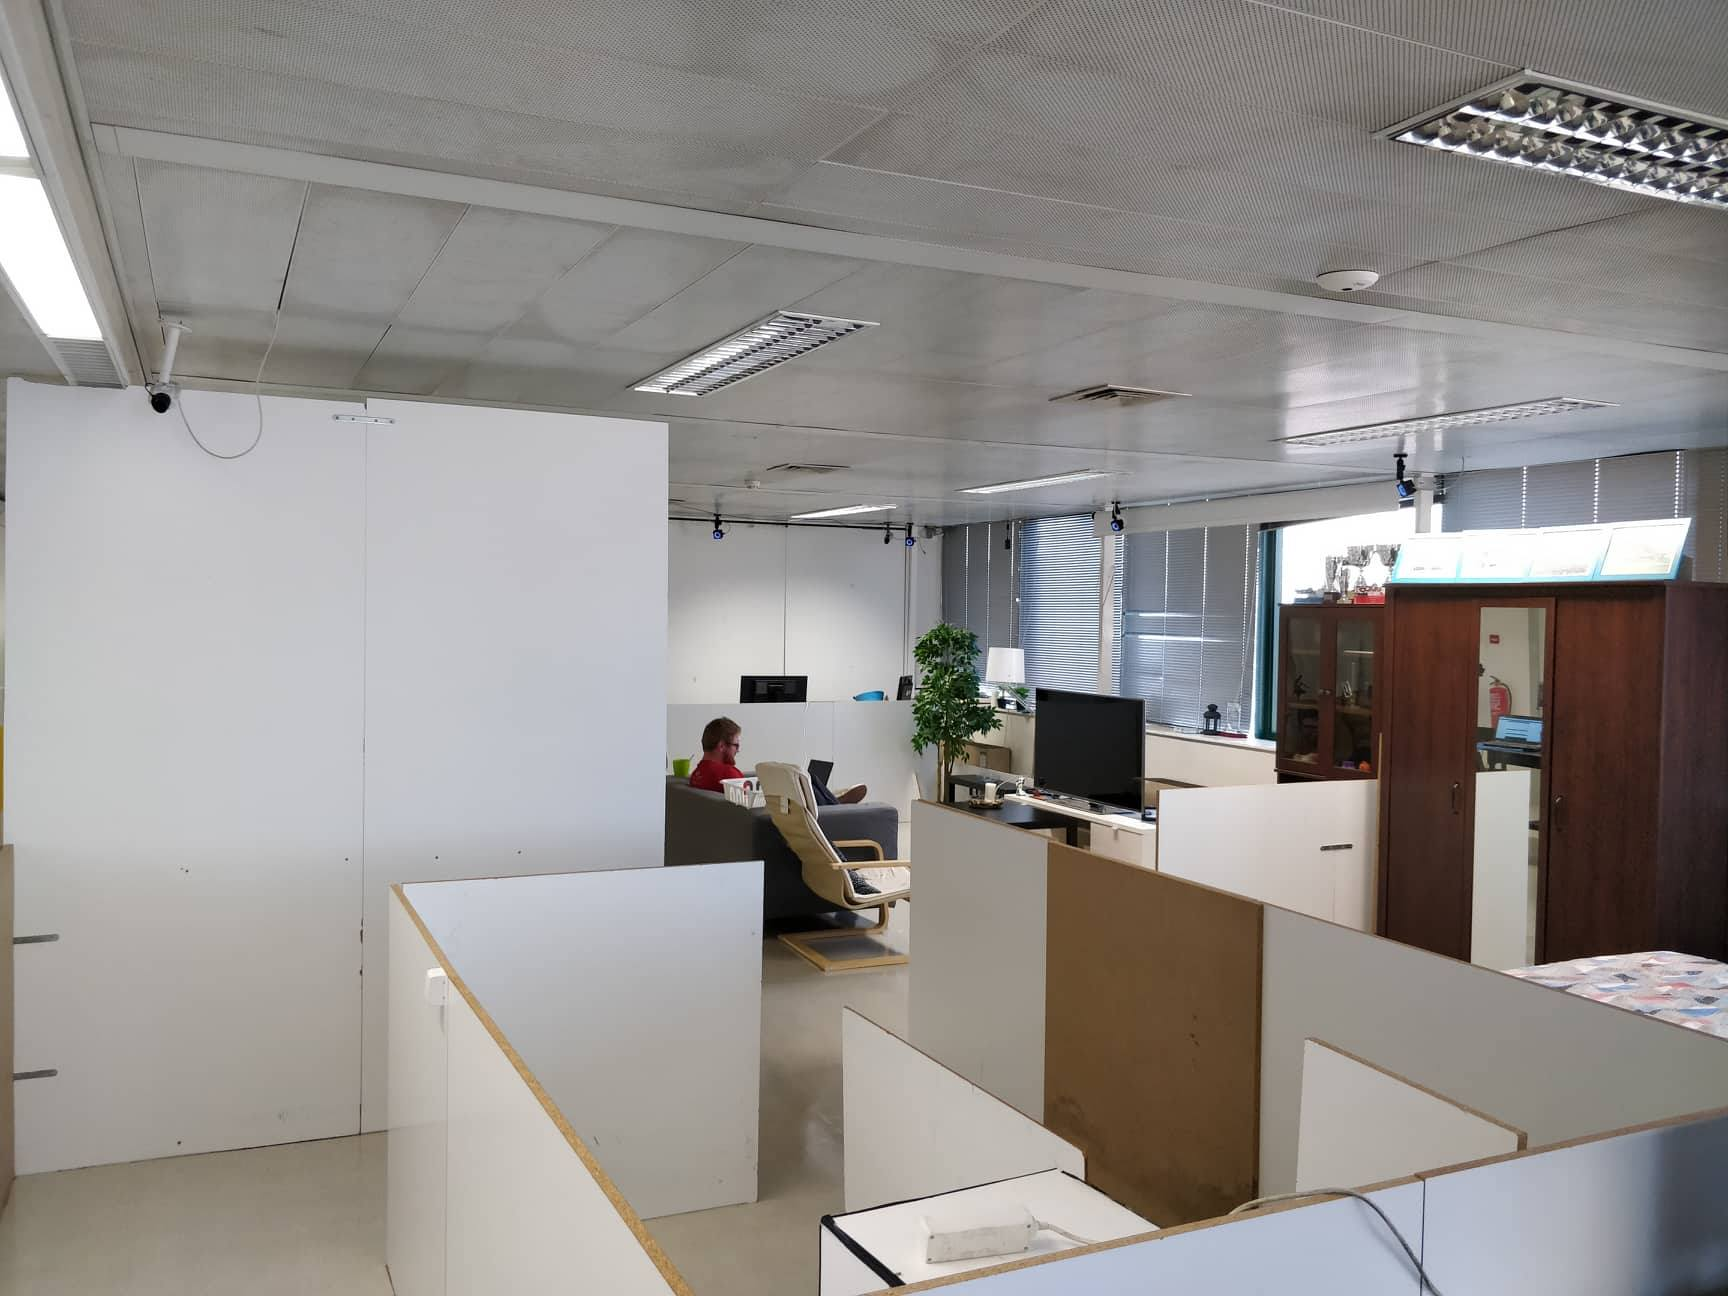
\includegraphics[width=0.8\linewidth]{images/41339074_481840472313432_6451621996257083392_n.jpg}
    \caption{SocRob@Home home laboratory}
    \label{laboratory}
\end{figure}


The subject of my internship was visual servoing on a 7\gls{DoF} arm. The goal is to control Mbot's arm with a  control law to make him able to grasp various types of object in various conditions.
In the next section, I am going to present my motivation and state the problem of my internship in this context and environment that we just presented.
\newpage


\section{Motivation}

Robust execution of complex manipulation tasks in dynamic environments is essential for service robots in domestic environments to assist their users in their daily tasks. By dynamic environment, I mean an environment that is changing, that could be known and unknown at the time (for the example the map of the apartment could be known but the position of the object to interact with could be unknown). Daily robotic tasks for a home robot on a manipulation side involve interaction with humans (shaking hands) and interaction with objects (taking an object from one position to a new one). Theses tasks involve the successful execution of multiple sub-tasks like object detection, grasping, carrying and placing objects.

Typically, object grasping problems are approached by using separate offline path planning and open loop execution methods, which expose some disadvantages. For instance, during trajectory execution, the robot is not sensitive to changes in the environment. If the target object pose is changed, the robot should ideally deal successfully with those situations and adjust accordingly. Having a control scheme that is closed loop will able the robot to adapt his movements to his dynamic environments.

A second problem when it comes to object grasping is related with robot base-camera-arm calibration. This work is motivated by the possibility of bypassing the calibration issues. Indeed, this work implied having a depth camera fixed on the end-effector and computing directly the visual control law in the image space, \gls{IBVS}.

A third problem is the variability of objects that the robot has to grasp. This work is motivated by the possibility to have a generic control law including a generic perception  for various types of objects and not restrained as a specific object.

\section{Problem Statement}

The problem is defined as the design and implementation of a generic real-time closed-loop image based visual servoing controller in a dynamic environment. This problem can be break down in three sub-sections: 

\begin{figure} [!h]
    \begin{minipage}[b]{0.5\linewidth}
        \begin{enumerate}
            \item Perception
            \begin{enumerate}
                \item Detection
                \item Features Extraction
                \item Tracking 
            \end{enumerate}
                \item Control Law
            \begin{enumerate}
                \item \gls{IBVS}
            \end{enumerate}
            \item Execution
            \begin{enumerate}
                \item Arm controller
            \end{enumerate}
        \end{enumerate}
    \end{minipage}
    \begin{minipage}[b]{0.5\linewidth}
      \begin{center}
        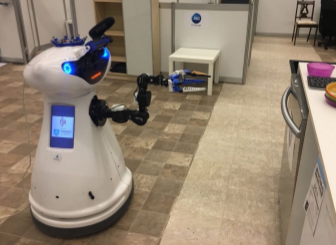
\includegraphics[width=0.8\textwidth]{images/mbot_grasping.png}
      \end{center}
      \caption{Mbot, in a grasping approach}
    \end{minipage}
\end{figure}

\newpage


This method has been applied for a domestic robots in a domestic environment. It has been both implemented in simulation and inside the real robot.

The closed loop controller take as input image, where characteristic features of the desired grasping object are extracted, with a perception part that has been developed from state of the art solutions. The camera velocities are computed as output since the camera is directly fixed on the end-effector we can assume that the end effector velocities are computed. 


\section{Report Outline}

This work has the following structures: Chapter \ref{chapter:Background} provides a state of the art review combined with background information required to understand the proposed solution. Chapter \ref{chapter:Controller_Design} presents the new approach, the implementation in simulation and inside the robot. Chapter \ref{chapter:conclusion} summarizes the achievements and discuss about future works. This chapter will also include a quick overview of the Portuguese life as requested. 

%!TEX root = ../dissertation.tex

\chapter{Background}
\label{chapter:Background}

This chapter provides fundamentals of theoretical knowledge required to understand the work for the previously stated problem. Firstly, we will discuss about object detection and feature extraction with presentation of the state of the art solution used (section \ref{Object_detection}). Secondly, we will describe the visual servoing control theory and solutions (section \ref{Visual_Servoing}). Thirdly, we will explain what is a manipulator in terms of robotics and what is kinematics of robotic manipulators (section \ref{Robotic_manipulator}).

\section{Object Detection and Features Extractions}
\label{Object_detection}

Object detection is the fist step performed by the presented controller. This detection is used to classify and track the object in real-time when the arm is moving (since the camera is fixed to the end effector) but also if the object is moved since the controller is used in a dynamic environment. Feature extraction is the second step performed by the controller and is used to compute the visual servoing control law.

\subsection{Objection detection}

Objection detection is a classical problem in computer vision, and it can be stated as recognize what the objects are inside a given image and also where they are in the image. To achieve this task, this work use a state of the art object detection algorithm called \gls{YOLO} \cite{DBLP:journals/corr/RedmonDGF15}.
\gls{YOLO} is a convolutional neural network that was introduced in 2015 and recently improved its accuracy and speed on object detection with YOLOv2 \cite{DBLP:journals/corr/RedmonF16}. It is an object detection system targeted for real-time processing. 

\subsubsection{Functioning}

The first step is given an image, YOLO starts by splitting that image into an n\*n grid cells (figure : \ref{pict:yolo_grid}). In this grid, each of the cells (in red, in figure \ref{pict:yolo_grid}) is responsible for predicting n bounding box associate with a confidence score. 

\newpage

\begin{figure} [!ht]
    \centering
    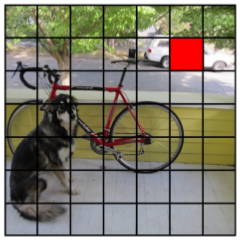
\includegraphics[width=0.4\linewidth]{images/yolo_grid.png}
    \caption{Image splitted into a n*n grid, from YOLO website}
    \label{pict:yolo_grid}
\end{figure}

Each individual bounding box confidence score tells you how certain YOLO is that the predicted bounding box actually contains an object and also how well the bounding box feats the object.

\begin{figure} [!ht]
    \centering
    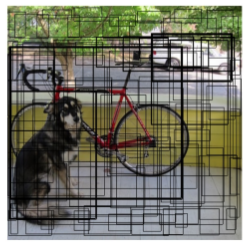
\includegraphics[width=0.4\linewidth]{images/yolo_confidence.png}
    \caption{Resulting prediction from all the grid cells (the thickness of the bounding box increase with the confidence, from YOLO website}
    \label{pict:yolo_confidence}
\end{figure}

In figure \ref{pict:yolo_confidence}, the prediction from all the cells regrouped together is visualized. This prediction take the aspect of many bounding box ranked by their confidence score. This way you know more or less where objects are in the image but you don't know what is the object.

The second step is for each cells (figure: \ref{pict:yolo_grid}) YOLO predicts a  class conditional probabilities. It only predicts one set of class probabilities per cell, regardless the number of bounding box associated with that cell. Note that since its using conditional probabilities, if a cell predict an object for example a bike it doesn't mean that inside of this cell there is this bike, it only means that if there is an object inside this bounding box then this object is a bike (figure \ref{pict:yolo_proba}).

\newpage

\begin{figure} [!ht]
    \centering
    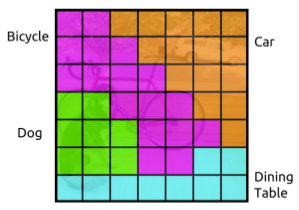
\includegraphics[width=0.4\linewidth]{images/yolo_proba.png}
    \caption{ Class conditional probability map from YOLO website}
    \label{pict:yolo_proba}
\end{figure}

The third step is to combine both previous step (confidence score for the bounding box and class conditional probabilities) into one final score. This final score evaluates the confidence that each bounding box contains a specific object (figure \ref{pict:yolo_final}).

\begin{figure} [!ht]
    \centering
    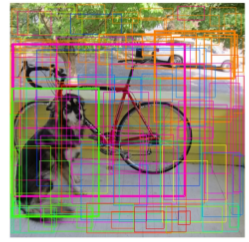
\includegraphics[width=0.4\linewidth]{images/yolo_final.png}
    \caption{Bounding box and class conditional probabilities, from YOLO website}
    \label{pict:yolo_final}
\end{figure}

In figure \ref{pict:yolo_final}, their are still a lot of bounding box, the only remained step is to filter this bounding box with a final score that has to be higher than a specific threshold. Also, duplicated bounding boxes are removed using a non-maximum suppression. The final result is visible on figure \ref{pict:yolo_final_filter}.

\begin{figure} [!ht]
    \centering
    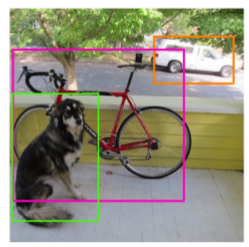
\includegraphics[width=0.3\linewidth]{images/yolo_final_filter.png}
    \caption{Final result after filtering, output from YOLO, from YOLO website}
    \label{pict:yolo_final_filter}
\end{figure}

\newpage

To summarize, each of the bounding boxes are composed by 5 predictions:
\begin{enumerate}
    \item x,y coordinates: offsets between the center of the bounding box relatives to the bounds of the cell.
    \item w,h: width and height of the bounding box
    \item confidence score, how YOLO is certain that this bounding box contains this object
\end{enumerate}

YOLO is a state of the art solution because it is a real time object detection system. What is the secret ? The output predictions are all computed at the same time looking only once the image (You Look Only Once). Since it predicts all of these detection simultaneously YOLO also implicitly incorporates global context in the detection process so it can learn things about which objects tend to occur together, the relative size and location of objects and other assorted things.

\subsubsection{Training}

YOLO is pre-trained on a ImageNet that is currently the biggest dataset for Computer Vision tasks (millions of images, more than a thousands class in different scenes). When pre-train, it learns to convert the millions images into a feature map (convolution weights). So when YOLO is actually trained with your own data set it adapts this convolutional weights to detect your own object class in the training set of images. Pre-train allows to have very good performance with a small training set. 

For the data augmentation, YOLO randomly scales and translates of up to 20\% of the original image size and also randomly adjusts the exposure and saturation of the image by up to a
factor of 1.5 and hue by up to a factor 0.1 in the HSV color space.

Overall the training of this network is straightforward and corresponds to a lot a of standards in the Computer Vision community: YOLO pre-train on ImageNet, uses stochastic gradient descent and uses data augmentation.

\begin{figure} [!ht]
    \centering
    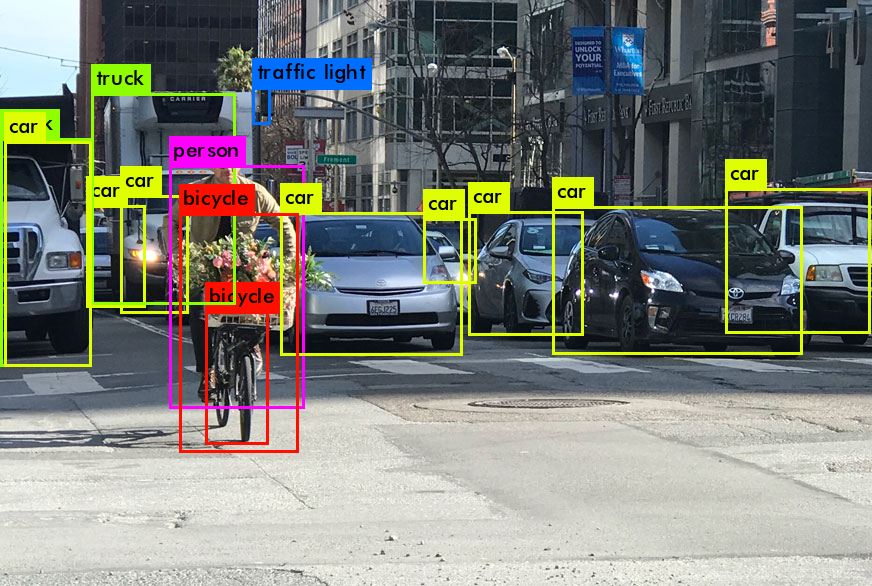
\includegraphics[width=0.65\linewidth]{images/yolo_example.png}
    \caption{YOLO at work, street road example}
    \label{pict:yolo_example}
\end{figure}


\newpage

\subsection{Feature Extraction}

Feature extraction is the second step performed by the presented controller.

\subsubsection{Image feature}

Image feature is a simple image pattern, based on which what we see in the image can be described. The main role of features in computer visions is to transform visual information into the vector space. On the vector space we will be able to apply mathematical operations on this features.
This features can be for example points, lines or ellipses.
The selected feature as what his called a feature parameter, it is any numerical quantity associated to the selected feature in the image plane. This can be coordinates of a point, angular coefficient and offset of a line, center and radius of a circle, generalized moments of an object in the image.

\subsubsection{Image Formation}

In this section, the image acquisition process will be described. To this purpose we will use the perspective camera model. It is the model the most commonly used in computer vision, it reproduces with the behaviour of real cameras with the most accuracy \cite{Szeliski:2010:CVA:1941882}.

\begin{figure} [!ht]
    \centering
    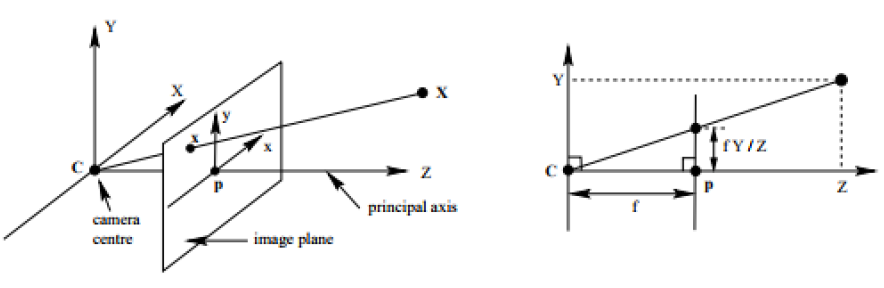
\includegraphics[width=0.65\linewidth]{images/model.png}
    \caption{Ideal pinhole camera model}
    \label{pict:pinhole_camera_model}
\end{figure}

Given a 3D scene in the world, a camera projects one or more 3-D point(s) onto the 2D image plane. The main feature of the perspective projection is the conservation of straight lines, after the transformation. The image formation can be described with a model called the pinhole camera model \cite{Hartley2004} (Figure: \ref{pict:pinhole_camera_model}).

Figure \ref{pict:pinhole_camera_model} shows the ideal representation of the pinhole camera model, considering a central projection of points in space, onto an image plan defined by $Z = f$ where $f$ is the focal length. The optical center $C$, located at the origin of this 3D coordinate system, represents the point in which all the 3D projection intersect. This principal axis is defined as the line perpendicular to the image plane, passing through the optical center. The principal axis intersects the image plane in the principal point $p$ \cite{Hartley2004}.

A point $X = (X,Y,Z)^T$ defined in the coordinate system of the camera, is mapped on the image, dividing the coordinates X and Y by the point depth Z, and multiplying by the focal length f as described in

\begin{equation}
    X = (X,Y,Z)^T = (f \frac{X}{Z},f \frac{Y}{Z})^T
    \label{eq_image_1}
\end{equation}
\newpage

Using homogeneous coordinates (\ref{eq_image_1}) can be written as:
\begin{equation}
   x = PX
\end{equation}
With $ x = (f \frac{X}{Z},f \frac{Y}{Z})^T $ and $ X = (X, Y, Z, 1)^T$ and the camera matrix P is composed by the matrix $K$ of intrinsic parameters and the extrinsic parameters matrix composed by the rotation matrix $R$ and the translation matrix $t$.
\begin{equation}
   P = K \big[ R|t \big]
\end{equation}
The matrix K of intrinsic parameters, also called calibration matrix can be represent as:
\[
K 
=
\begin{bmatrix}
    f_{x} & s & c_{x} \\
    0 & f_{y} & c_{y}\\
    0 & 0 & 1
\end{bmatrix}
\]
where $f_{x}$ and $f_{y}$ are independent focal length for the camera sensor x and y dimensions. $c_{x}$ and $c_{y}$ denotes the optical frame center expressed in pixel coordinates.

$X$ will be expressed in the camera coordinate frame but the points in 3D space are expressed in the world coordinate frame. The extrinsic parameters matrix (E)  represent the relation between this two spaces. It represents the external position and orientation of the camera in the 3D world and relates the camera frame to the world frame:
\[
E
=
\begin{bmatrix}
    R_{[3x3]} & t \\
    0_{[1x3]} & 1
\end{bmatrix}
\]
an homogeneous matrix composed by a rotation matrix (R) and a translation vector (t).\\

To resume, in this section we have been looking into general knowledge about image features and image formation. Object detection and feature extraction are the first step in the algorithm that will be describe in the next chapter.
\newpage
\section{Visual Servoing}
\label{Visual_Servoing}

\gls{VS} relies on techniques from areas like image processing, computer vision, and
control theory. Here, we present a definition of VS, Image-Based Visual Servoing (IBVS), \gls{PBVS}, and Hybrid method. Different ways of classifying these techniques are possible. Several classifications are extensively discussed in \cite{Staniak:2010:SVS:1831760.1831963}.
VS is the use of the vision to extract features and to process images to control robot pose. The introduction to visual feedback makes the system less sensitive to errors that could be generated by inadequate calibration, noise in the system or changes in the environment. Contrarily to open-loop approaches, like "looking" then "moving" methods, the use of visual information acquired in real time, makes the control scheme more robust and adaptive. VS, using visual-feedback control loop, increases the overall accuracy of the systems and appears as an attractive technique to achieve manipulation tasks.

When doing visual servoing two camera configurations are defined: EYE-IN-HAND and EYE-TO-HAND (figure:\ref{pict:eye_in_hand})
\begin{figure} [h]
    \centering
    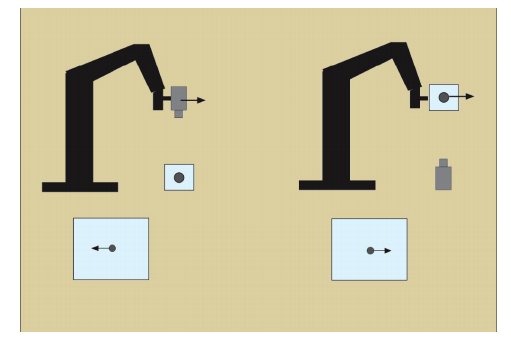
\includegraphics[width=0.65\linewidth]{images/eye_un_hand.png}
    \caption{EYE-IN-HAND (on the left) and EYE-TO-HAND (on the right) configuration}
    \label{pict:eye_in_hand}
\end{figure}\\
Based on \cite{<inria-00350283>}, we will describe the various basic approaches in \gls{VS}. 

\subsection{Image Base Visual Servoing}
\label{chap:ibvs}

IBVS uses measurements in the image m(t) (pixel coordinates, lines, moments
of region,...) converted to features using camera intrinsic parameters
p. The error signal is measured directly from the image. The control law is
based on the computed error between the set of current visual features and the set of 
desired features given by $s^*$. The interaction matrix relates a 2D point projected in
the image from a 3D point in the camera frame, by the depth of the point in
the camera frame
The error is defined as:
\begin{equation}
\label{first_ibvs}
e(t)=s(m(t),p) - s^*
\end{equation}
with m(t), the computation from the image measurements, e.g. image coordinates of interest point, area, center of gravity.
p, other parameters like camera intrinsic parameters, 3D models of objects or the pose between camera and environment.
The time variation of $s$, $\Dot{s}$ and the camera spacial velocity, $v_{c}$ has been related by Chaumette in \cite{<inria-00350283>} like:

\begin{equation}
    \Dot{s} = L_{s}v_{c}
    \label{equation_1_ibvs}
\end{equation}
with $v_{c} = (v_{c}, w_{c})$, describing linear velocities and angular velocities relative to the origin of the camera frame.
$L_{s}$, is  called the interaction matrix (k, number of visual features * N, number of robot DoF).

The time variation of the error is equal to the time variation of the current features:
\[
\Dot{e} = \Dot{s}
\]
From \ref{equation_1_ibvs}, we can relate the time variation of the error with the precedent relation:
\begin{equation}
     \Dot{e} = L_{s}v_{c}
     \label{equation_2_ibvs}
\end{equation}
The goal is to reduce the error, to make the error converge to a lower value, to achieve this purpose an exponential decay was introduced \cite{<inria-00350283>} :
\begin{equation}
     \Dot{e} = - \lambda e
\end{equation}
From \ref{equation_2_ibvs} and since the control is done on the camera velocities the control law becomes:
\begin{equation}
\label{eq_control_law}
    v_{c}= - \lambda L_{s}^+ e
\end{equation}
with $L_{s}^+$ the Moore-Penrose pseudo inverse matrix, that is defined as:
\[
L_{s}^+ = (L_{s}^T L_{s})^{-1} L_{s}^T
\]
when $(L_{s}^T L_{s}$ is of full rank. Both $L_{s}^T$ and $L_{s}$ are hard to be exactly computed in real \gls{VS} systems. They have to be estimated as $\hat{L_{s}}$ in the control law. 

From a 3D point coordinates (X,Y,Z) and related to the image formation subsection, the point coordinates are defined in the image plan as:
\begin{equation}
    \begin{aligned}
    x = X / Z \\
    y = Y / Z
    \end{aligned}
\end{equation}
From this point coordinates, the current features and desired features are constructed: 
\begin{equation}
    \begin{aligned}
     s = (x, y)\\
     s^* = (x, y) 
    \end{aligned}
\end{equation}
Now, the time variation of the previous point coordinates can be written as:
\begin{equation}
\label{eq1_interaction}
    \begin{aligned}
    \Dot{x} = (\Dot{X} - x\Dot{Z})/Z \\
    \Dot{y} = (\Dot{Y} - y\Dot{Z})/Z
    \end{aligned}
\end{equation}
Relating the velocity of the 3D point with the camera spatial velocity is given by:
 \begin{equation}
 \label{eq32_interaction}
    \Dot{X} = - v_c - w_c * X
 \end{equation}
Becomes:
\begin{equation}
\label{eq2_interaction}
    \begin{aligned}
    \Dot{X} = - v_x - w_y * Z + w_z*Y \\
    \Dot{Y} = - v_x - w_y * Z + w_z*Y \\
    \Dot{Z} = - v_x - w_y * Z + w_z*Y
\end{aligned}
\end{equation}
Now using (\ref{eq2_interaction}) inside (\ref{eq1_interaction}):
\begin{equation}
\label{eq3_interaction}
    \begin{aligned}
    \Dot{x} = - \frac{v_x}{Z} -(1+x^2)w_y + w_z y + \frac{x}{Z} v_z + x y w_x \\
    \Dot{y} =- \frac{v_y}{Z} + (1+x^2)w_x + w_z x + \frac{x}{Z} v_z - x y w_y \\
\end{aligned}
\end{equation}
\ref{eq3_interaction} can be written as:
\begin{equation}
    \Dot{x} = L_x v_c
\end{equation}
Finally, the interaction matrix related to the 3D point is:
\[
\begin{bmatrix}
    - \frac{1}{Z} & 0 & \frac{x}{Z} & x y & -(1+x^2) & y \\
    0 & - \frac{1}{Z} & \frac{y}{Z} & 1+y^2 & - x y & x 
\end{bmatrix}
\]
If more than one point is used, the global interaction matrix will be stacking intermediate interaction matrix. For example if 3 points are used $x = (x_1, x_2, x_3)$:
\[
L_x
=
\begin{bmatrix}
    L_{x1} \\
    L_{x2} \\
    L_{x3} 
\end{bmatrix}
\]

This matrix has to be estimated when used in control law and the quantity of points chosen has to be enough to avoid singular configurations and local minima.
They are several methods to estimate the interaction matrix in IBVS \cite{<inria-00350283>}. 

The most straight forward method is to estimate the current depth Z of each point, at each iteration of the control scheme:
\[
\Hat{L_s^+} = L_s^+ 
\]
According to \cite{<inria-00350283>}, this method gives a good local behavior but the global behavior is unsatisfactory. It means that the convergence will not be as good as expected.

Another approach is to set only the desired depth $Z^*$ of each point for the desired pose:
\[
\Hat{L_s^+} = L_{s^*}^+ 
\]
According to \cite{<inria-00350283>}, this method gives a good local behavior but introduce unexpected translational motion. 

A minimization approach as lately been proposed \cite{1308092} leading to chose:
\[
\Hat{L_s^+} = \frac{1}{2}(L_{s^*}^+ + L_s^+)
\]
This method gives a better trajectory with less oscillations. \\

Problems from using a \gls{IBVS} are referred in literature, like problems of singularities in the interaction matrix, or the reach of local minima can lead to problem in the control. It is also known as a highly coupled process. A correct estimation of the interaction matrix in IBVS is important to provide stability to the control system and avoid perturbations. 

\subsection{Pose Based Visual Servoing}
\label{chap:pbvs}

\gls{PBVS} uses 3D features instead of 2D, as in IBVS, required to estimate the
pose of the targeted object. Features are extracted from the image and used to
determine the pose of the target with respect to the camera, in the Cartesian space \cite{<book-coork>}. Various methods of 3D pose computation of an object exist in the literature from triangulation methods, to model based estimation. The classical computer vision problem is called the 3D localization problem \cite{LOWE1987355}. Once the 3D reconstruction of the object is established, the error is then computed in the task space and used in the control law.
All the previous step of the control law computation from (eq: \ref{first_ibvs}) to (eq: \ref{eq_control_law}) presented in the previous section are still valid. However, the interaction matrix will not be the same. \\

Four coordinate frames are considered: the current camera frame $C$, the world base frame $W$, an object frame $O$, as reference of frame of the object and  a desired camera frame $C^*$. The orientation of $C$ relative to $C^*$ is given by a rotation matrix $R_{[3x3]}$. The corresponding angle parametrisation $\theta$ and the translation vector t, defines the feature s.
The computation of the interaction matrix will then depend on how t is defined:

If t is defined as a function of $O$, $t^C_O$, $\theta = 0$ for the desired feature $s^*$  and the error is computed between  $t^C_O$ and $t^{C^*}_O$
\[
L_e
=
\begin{bmatrix}
    -I_3 & t \\
    0 & L_\theta
\end{bmatrix}
\]
with $I_3$ the identity matrix.
If t is defined as a function of $C$, $t^{C^*}_O$, $m^* = 0$ and $e=s$, the interaction matrix will be:
\[
L_e
=
\begin{bmatrix}
   R^{C^*}_C & 0 \\
    0 & L_\theta
\end{bmatrix}
\] \\

Usually the trajectory is better followed in 3D space than in image space due to the definition in Cartesian space. However, points can leave the image space due to the fact that the control is not directly done in the image. In PBVS a correct estimation of the pose is crucial, because of the error regulation. So the 3D reconstruction depends directly on the calibration of the vision system.

\begin{figure} [!ht]
    \centering
    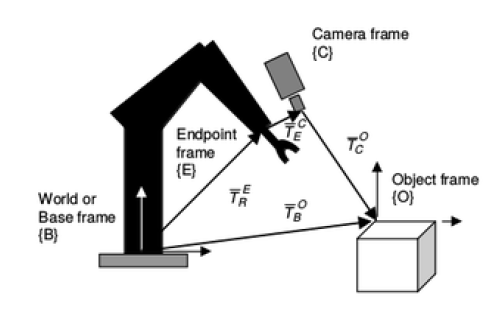
\includegraphics[width=0.5\linewidth]{images/coordinates_frame_pbvs.png}
    \caption{PBVS, coordinate frames overview}
    \label{pict:pbvs}
\end{figure}

\subsection{Hybrid}

In the two previous sections, the two main methods for \gls{VS}, where presented. A combination of these methods is also possible, it is called Hybrid visual servoing. The basic idea behind hybrid visual servoing is to decouple the Z axis motions (including
both the translational and the rotational components) from the other DoF. In this section, one method of hybrid visual servoing will be presented but it is not the only possibilities, more methods are present in the literature. 
The 2-1/2D visual servoing is an hybrid method. The main idea is to control the camera motion with both IBVS and PBVS. IBVS will be use to control the translational motion and PBVS to control the rotational motion. In \cite{<inria-01350283>}, starting from the hypothesis that a control for angular velocity $w_c$ is available, in PBVS method can be defined as:

\begin{equation}
    w_c = - \lambda \theta
\end{equation}
The goal is to control the several translational DoF by partitioning the interaction matrix into two matrices: $L_v$, matrix of linear velocities, and $L_w$, matrix of angular velocities, obtaining:
\begin{equation}
    L_e
=
\begin{bmatrix}
   L_v & L_w \\
    0 & L_\theta
\end{bmatrix}
\end{equation}
Now, the time variation of the feature can be describe as:
\begin{equation}
    \Dot{s}
=
\begin{bmatrix}
   L_v & L_w 
\end{bmatrix}
\begin{bmatrix}
   v_c \\ 
   w_c
\end{bmatrix}
\end{equation}
The desired translation control input is solved for an error with an exponential decay:
\begin{equation}
    \Dot{e_t} = -\lambda e_t
\end{equation}
At the end, the following control law is obtained to express the translational motion input:
\begin{equation}
    v_c = - L_v^+(\lambda e_t + L_w w_c)
\end{equation}
 with $\lambda e_t + L_w w_c$, the new error expression. \\

To resume, in this method, the translational velocities are computed from an IBVS control law and the rotation velocities can be added later using a 3D pose estimation algorithm and compute using PBVS visual servoing. 


\section{Robotic manipulators and kinematics}
\label{Robotic_manipulator}

Robotic servo manipulators are kinematic chains.They are composed of links, and this links are connected by joints (figure: \ref{pict:chain}). The fixed part of the chain is called the base and the ending part is called the end effector. It is where usually the tool performing the task (effector) is fixed, for example a gripper. In robotic manipulators joints are the movable elements, which enable relative movement between the neighboring links. \\

\begin{figure} [!ht]
    \centering
    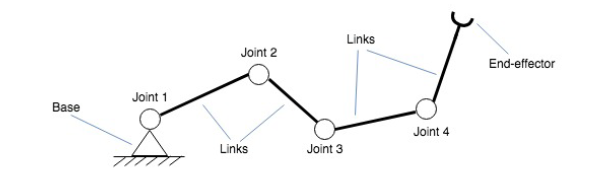
\includegraphics[width=0.65\linewidth]{images/chain.png}
    \caption{Kinematic chain of manipulator}
    \label{pict:chain}
\end{figure}

To describe the position and orientation of the robotic manipulator in space, frames are attached to the links and to the end effector (figure: \ref{pict:frames}). Each frame is expressed with respect to a reference frame called base frame. Description of the frame is given by position vector (position description) relative to some other reference frame and rotation matrix (orientation description).

\begin{figure} [!ht]
    \centering
    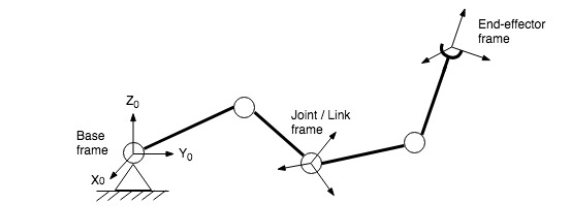
\includegraphics[width=0.65\linewidth]{images/frames.png}
    \caption{Frames attached on the manipulator joints}
    \label{pict:frames}
\end{figure}
This transformation is stored in an homogeneous matrix:
\[
T
=
\begin{bmatrix}
    R_{[3x3]} & t \\
    0_{[1x3]} & 1
\end{bmatrix}
\]

To compute transformation between base frame and last link, kinematic equations are use. For example, the transformation from frame {i} to frame {0} (base frame) can be written:

\begin{equation}
    T_i^0=T_1^0 T_2^1 ... T_i^{i-1}
\end{equation}
The transformation is a function of all joint variables and it computes Cartesian position and orientation of the last link frame.

\subsection{Forward kinematics}
\label{chap:forwardkinematics}


Knowing simple geometrical manipulator’s frames positions, in respect to other adjacent frames, it is possible to compute coordinates of the end effector, from the given joints angles. In other terms, using kinematic equations of the robot, it is possible to compute the position of the end effector from specified value of the joint parameters. This is referred as forward kinematics \cite{trove.nla.gov.au/work/27361264}.
Considering the system parametrization in figure \ref{pict:dh}:

\begin{figure} [!ht]
    \centering
    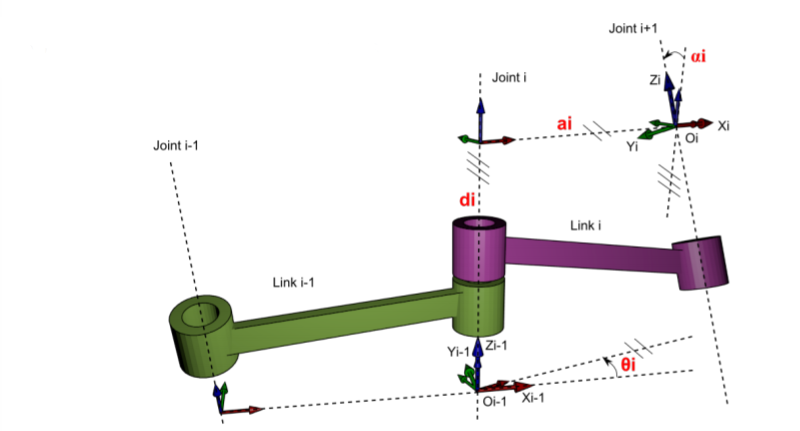
\includegraphics[width=0.45\linewidth]{images/dh.png}
    \caption{Robotic manipulator, with DH parametrization}
    \label{pict:dh}
\end{figure}

To compute forward kinematic problem, the Denavit-Hartenberg convention is usually used. This convention defines a transformation between frame {i} relative to the frame {i-1}. The general form of $T_i^{i-1}$:

\begin{equation}
    A_i = Rot_{z,\theta _i} Trans_{z,d_i} Trans_{x,a_i} Rot_{x, \alpha _i}
\end{equation}
with $A_i$, the transform between a link i and its parents i-1.
\begin{enumerate}
    \item z-axis of parent link i-1 aligned with axis of joint i
    \item 4 parameters for joint angle ($\theta _i$), link offset ($d_i$), link length ($a_i$), link twist ($\alpha _i$)
\end{enumerate}
Solving this transformation from base link to end effector link, the pose of the end effector can be compute what solves the forward kinematic problem. 

\subsection{Inverse kinematics}
\label{chap:inversekinematics}


Another method to control the pose of the end effector is the inverse method of the forward kinematic called inverse kinematic \cite{trove.nla.gov.au/work/27361264}. The inverse kinematics method calculates a set of all possible joints angles, which can be used to obtain desired position and orientation of the end effector. In terms of Denavit-Hartenberg convention, we are searching for an angle ($\theta _i$) with given $T_i^{i-1}$. In case of obtaining multiply solutions, decisions has to be taken to have an optimal motion in terms of various factors and constraints.
There is also possibility of nonexistence of the problem solution. It also might be state that point is not reachable for the manipulator. This method is subject to singularities, for example there are an infinite solution to reach the desired pose and the robot is lost on the one to choose. Local minima is another issue, the manipulator think that the pose has been reached but it is not, it is just a local minima. Finding the correct solution might be more complex than when using forward kinematics. They are a lot of different methods to solve inverse kinematic problems such as iterative methods or closed loop methods for example \cite{326569}.

The iterative methods solve the inverse kinematics problem by using a sequence of attempts leading to incrementally better configuration for the joints angles. Achieving better configuration means minimizing the difference between the current and target positions of the robot’s end-effector.

Another approach is closed-form method. In a closed-form method, the solution of the joints angles configuration can be straightforward expressed as a set of closed-form equations. Closed-form method gives a clear, single solution when is used for 6-degree-of-freedom systems with special kinematic structure
of kinematic chains

For mapping the joint velocities to the spatial velocities of the end effector expressed in word frame, the Jacobian matrix is used. For the work presented here, it is used given an end effector spatial velocity vector to compute the joint velocities to achieve this command as long as the Jacobian is non-singular.

\begin{equation}
    v_c = J(X) \Dot{\theta }
\end{equation}
with $v_c$, vector of spatial velocities and $\theta$, joint angles. 
\newpage
%TEX root = ../dissertation.tex

\chapter{Implementation}
\label{chapter:Implementation}

In this chapter, the first section \ref{Previous_architecture} will be about the previous control architecture, divided in subsections describing the previous open loop control scheme and describing the one developed at the same time by another student based on \gls{PBVS}. The second section \ref{developed_solution} is about the  design and implementation of the developed solutions, it will be divided in four subsections, the first one is about describing the approach, the second one is about the hardware and software tools used for this work, the third one is about the implementation of the first solution and fourth one is about the final implementation.

\section{Previous architecture}
\label{Previous_architecture}
\subsection{Open-loop}
The implemented system used before I began my work was an open loop control scheme (figure:\ref{pict:open_loop}). Once the trajectory is planned, execution module does not considering possibility of goal object movement or unexpected obstacles. In this approach robot is “blindfolded” what gives several drawbacks specially accuracy and reliability since the system does not have feedback on the control.
\begin{figure} [!ht]
    \centering
    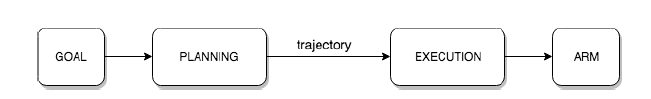
\includegraphics[width=0.75\linewidth]{images/open_loop.png}
    \caption{Open loop architecture}
    \label{pict:open_loop}
\end{figure}

Trajectory is planned, from the current pose to the desired pose, before the manipulator starts its motion. Execution is realized by a trajectory controller from Moveit! framework. The following module takes computed trajectory, which is a sequence of joints angles, converts them into the drivers speed and sends information to the servos of manipulator. 

\subsection{PBVS}

During the period of my internship, another student was working at the time, on the development on a new controller for the arm. This work was based on developing an optimization based Cartesian controller for the arm (from an input desired pose and the current position of the end effector computing joint velocities to reach the desired pose with constraints on joint position). Combining this work with a pose estimation algorithm developed by another student using also YOLO, a \gls{PBVS} is implemented (\ref{chap:pbvs}). It is using the head camera of the robot, so an EYE-TO-HAND configuration (figure:\ref{pict:eye_in_hand}).
\begin{figure} [!ht]
    \centering
    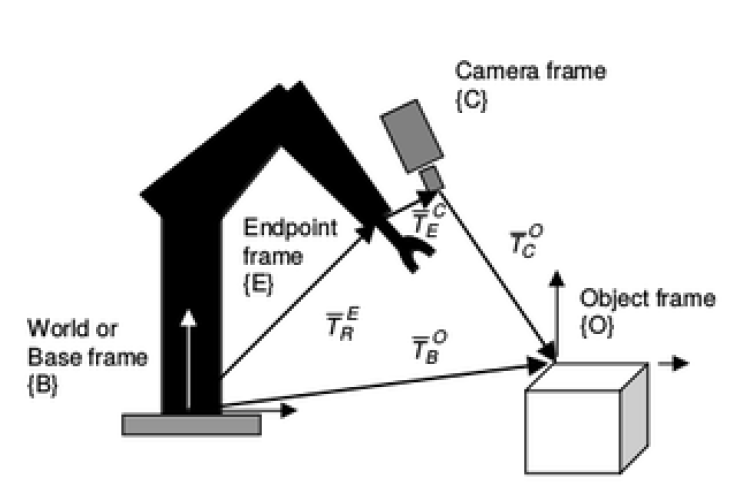
\includegraphics[width=0.95\linewidth]{images/pbvs.png}
    \caption{PBVS architecture developed by another student}
    \label{pict:pbvs_emilia}
\end{figure}

This controller is combining motion of the base and the arm. It has been designed as an optimization problem. For now, it applied constraints to avoid joint limits.

\section{Developed solutions}
\label{developed_solution}

\subsection{Approach}
Applying an Image Based Visual Servoing control law to Mbot 7DoF with an EYE-IN-HAND configuration is the subject of this work. This title is describing the working approach. The approach here is to use an \gls{IBVS} (\ref{chap:ibvs}). This control law is applied to a robotic manipulator that has 7 joints and 7\gls{DoF}. The camera is fixed on the end effector that is defined as an EYE-IN-HAND configuration (figure: \ref{pict:eye_in_hand}).
\subsubsection{Constraints}
The constraints for this work are:
\begin{itemize}
    \item Using an IBVS control law with an EYE-IN-HAND configuration
    \item No predefined object, the algorithm as to be as generic as possible
    \item The algorithm has to as close as real time as possible
    \item The working environment is not fixed, it is dynamic, the control law has to adapt to new environment and if the object move during the grasping approach
    \item Having a grasping approach, not only going to a certain pose but also think about grasping
\end{itemize}
\subsubsection{Why using an \gls{IBVS}}
The two major benefits of using an \gls{IBVS} in a grasping approach are:
\begin{itemize}
    \item Avoiding calibration issues, the precision for grasping is really important, because a small error (cm) can lead to a grasping fail.
    \item Closed loop and able to be use in a dynamic environment
\end{itemize}
In the next subsection, the tools used for this work will be described hardware and software.

\subsection{Hardware and Software}
To achieved the design and implementation of the previously described approach, we did not start from scratch. We used existing libraries, software and also of course an already very advanced robot  hardware speaking robot, Mbot.
\subsubsection{Software}
\begin{itemize}
    \item 
\gls{ROS} is a middleware (\ref{pict:ros}). It is a computer software that provide services to software applications. It makes easier for software developers to implement communication and input/output, so they can focus on the specific purpose of their application.
\gls{ROS} is a flexible framework helping developers creates software for robots \cite{288}. It provides device drivers, collection of tools and libraries, visualizers, message-passing, package management, and more to simplify the task of creating complex applications across various robotics platforms. ROS is licensed under an open source. Developed controller is implemented in the Robot Operating System environment for the needs of integration the module with the team code base.
\begin{figure} [!ht]
    \centering
    
\includegraphics[width=0.35\linewidth]{images/ros.png}
    \caption{Robot Operating System, since 2007.}
    \label{pict:ros}
\end{figure}

    \item
\gls{ViSP} is a modular C++ library that allows fast development of visual servoing applications \cite{articlevisp}. ViSP is developed and maintained by the Inria Rainbow (former Lagadic) team located at Inria Rennes. The platform takes the form of a library which is divided in several modules (core, io, gui, vision, …). ViSP software environment features independence with respect to the hardware, simplicity, extendibility, and portability. ViSP also features a large library of elementary tasks with various visual features that can be combined together, an image processing library that allows the tracking of visual cues at video rate, a simulator, an interface with various classical framegrabbers, a virtual 6-DOF robot that allows the simulation of visual servoing experiments, etc. The platform is implemented in C++ under Linux.

To use ViSP inside a ROS environment, ViSP ROS package was used. It also have been developped by Inria Renne. It is an extension of the ViSP library. While ViSP is independent from ROS, in $visp_ros$ we benefit from ROS features.
\begin{figure} [!h]
    \begin{minipage}[b]{0.5\linewidth}
        \begin{center}
            
\includegraphics[width=1\linewidth]{images/bandeauViSP.png}
        \end{center}

        \label{pict:visp_logo}
    \end{minipage}
    \begin{minipage}[b]{0.5\linewidth}
      \begin{center}
        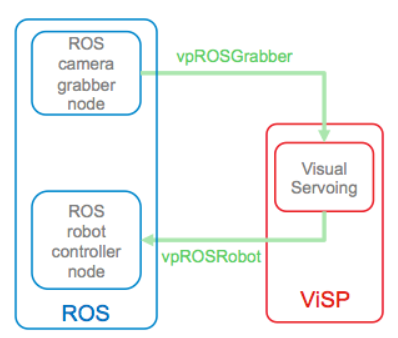
\includegraphics[width=0.8\textwidth]{images/visp_ros.png}
      \end{center}
    \end{minipage}
    \caption  {ViSP, Visual Servoing Plateform, developed by Inria Renne, 2005}
\end{figure}

    \item 
Gazebo is a simulation software that is highly compatible with ROS development. Robot simulation is an essential tool in every roboticist's toolbox. A well-designed simulator makes it possible to rapidly test algorithms, design robots, perform regression testing, and train AI system using realistic scenarios. Gazebo offers the ability to accurately and efficiently simulate populations of robots in complex indoor and outdoor environments.Gazebo is an open source software, improved by the community.
\begin{figure} [!h]
    \begin{minipage}[b]{0.4\linewidth}
        \centering
        
\includegraphics[width=1\textwidth]{images/gazebo.jpg}
    \end{minipage}
    \begin{minipage}[b]{0.6\linewidth}
      \begin{center}
        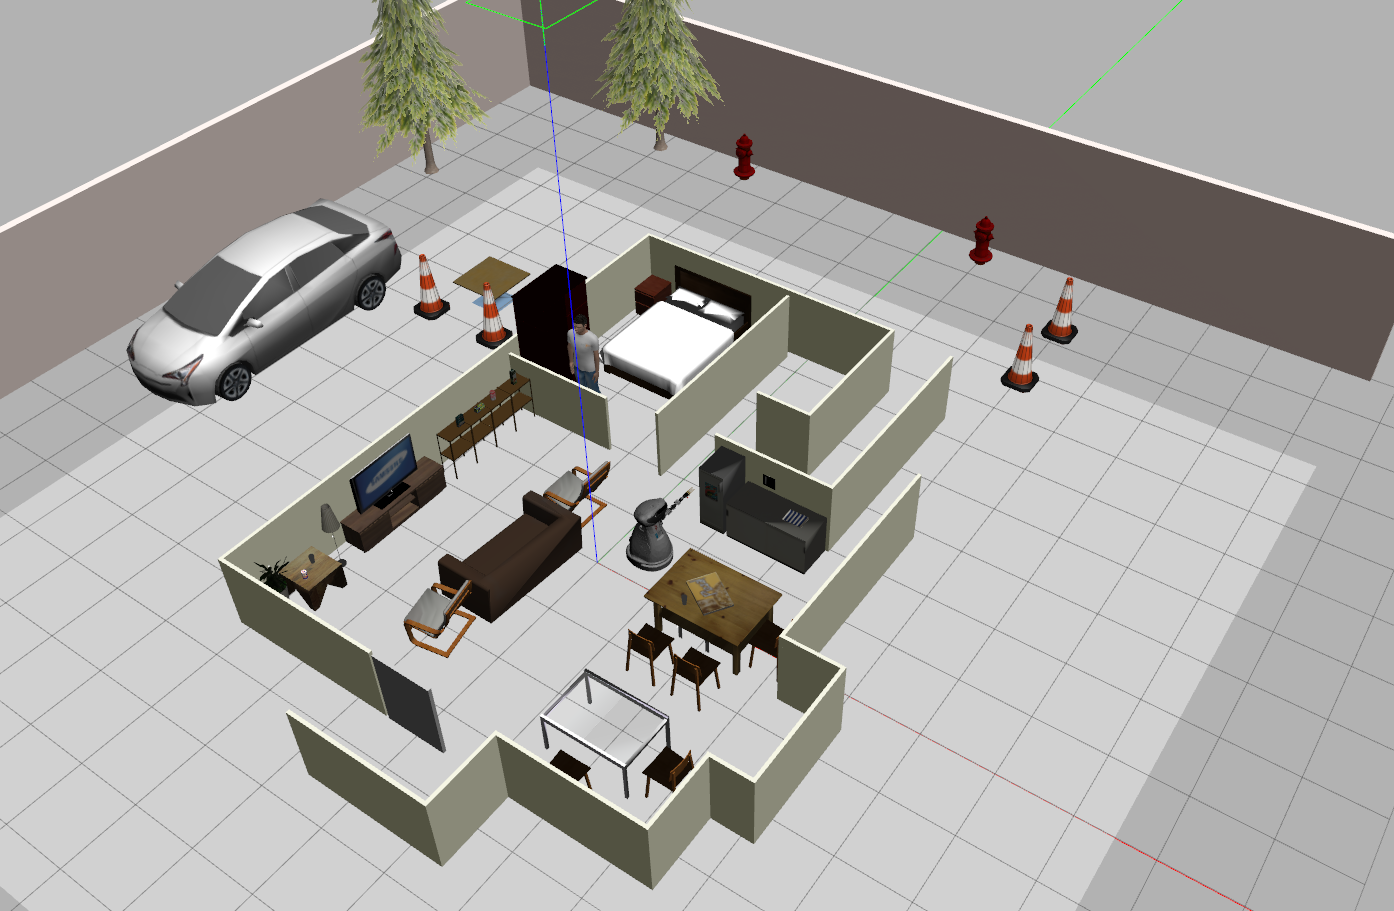
\includegraphics[width=0.8\textwidth]{images/gazebo_isr_testbeld.png}
      \end{center}
    \end{minipage}
    \caption{Gazebo, ROS friendly simulation software(left), ISR testbeld used to test robot tasks in Gazebo (right)}
\end{figure}
    \item 
\gls{URDF} is a package of a number of XML format files, used in \gls{ROS} to describe all elements of the robot. XML files contain specification of sensors, robot models, scenes and more. Each file of XML format has a corresponding in one or more programming language parser. In our project the URDF files contains the most essential information for this work about manipulator (number of joints, links lengths, joints limits, etc.) as well as information about the robotic base. It is also used to construct the robot model in Gazebo for example and in Rviz.
    \item 
\gls{YOLO} is a convolutional neural network used in this work to detect and extract features. It has been described in the the chapter \ref{chapter:Background} in section \ref{Object_detection}.
    \item 
Controlling arm servos (sending commands to the joints of the arm), to this purpose two possibilities:
    \begin{enumerate}
        \item  An inverse kinematic controller, that take as input a desired velocity vector of the end effector and compute the corresponding joint velocities to achieve the desired velocity for the end effector. This "controller" only controls the arm and not the arm and the base of the robot combined to be able to reach a larger area when having a grasping approach. The well known problem when using inverse kinematic as described in section \ref{chap:inversekinematics} is singularities and local minima.
        \item An optimization forward kinematic controller, developed during the time of my internship to use with his work on \gls{PBVS}. This "controller" controls the arm and the base at the same time. It takes as input a pose in world frame and output the joint velocities, more information on the section \ref{Previous_architecture}. Since it is an early development many problems appeared using this controller, like when doing the optimization not using the last joint or not taking as input velocities. One of my work was to convert this controller to be able to end effector velocities as input.
    \end{enumerate}

\end{itemize}


\subsubsection{Hardware}
\begin{itemize}
    \item Cython Gamma 
    \item Intel realsense D435 depth camera
\end{itemize}

In the next subsections we will present the developed solutions. The work will be divided in two part: a first solution and a final solution. When I start my internship, the robot was not equipped with a camera fixed on the arm effector. Also before implementing your algorithm, it is usual to first test it inside a simulated environment. The first implementation has been developed in simulation and the final solution has been implemented in simulation and inside the real robot. The main difference between these solutions is the way its initialized and the way the features are detected and extracted.

\subsection{1st solution}
  
The first solution is based on a simple feature detection and tracking method called blob detection and tracking. Blob detection methods aimed at detecting regions in an image that differ in properties such as color, brightness for example compared to surrounding regions. Informally, a blob is a region of an image in which some properties defined by the user are constant or approximately constant. In simulation this blob are black point a juice box.\\
The control scheme of this first implementation is described in the figure: \ref{pict:control_scheme_1}.
\begin{figure} [!h]
    \centering
    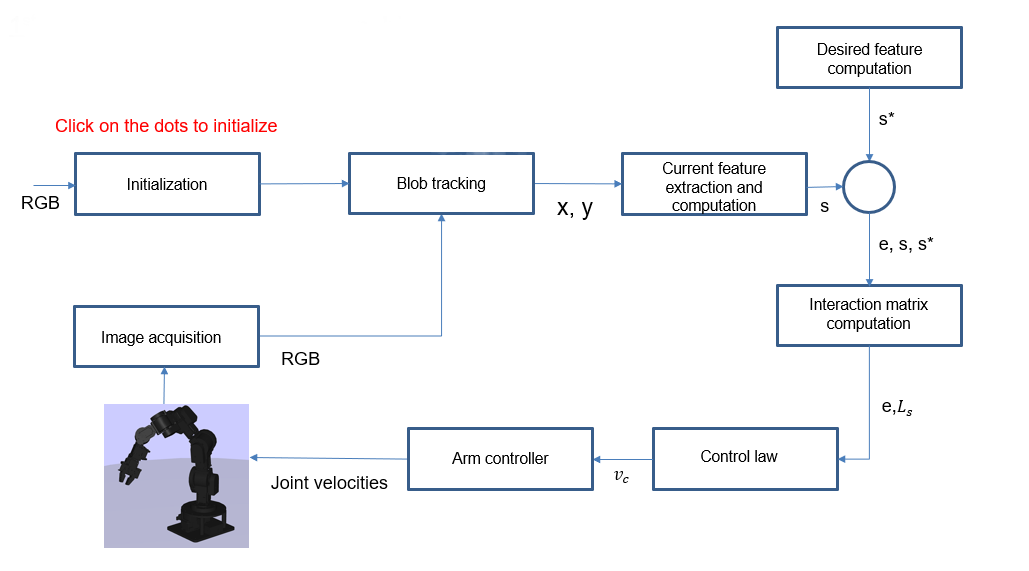
\includegraphics[width=1.\linewidth]{images/control_scheme_1.png}
    \caption{First implementation control scheme}
    \label{pict:control_scheme_1}
\end{figure}

The first step of this control scheme is the initialization, the user as to click with the mouse inside the display on the 4 dots. 



interaction matrix 2 parameters
scheme
pro cons

\subsection{Final solution}
interaction matrix 3 parameters
scheme
pro cons

\section{Implementation}
\label{implementation}

\subsection{Solutions}
\subsubsection{Hardware}
cython arm
intel cam

\subsubsection{Software}
gazebo
ROS
visp
visp ros
YOLO

\subsection{Results}

\subsubsection{1st implementation}


\subsubsection{Final implementation}




%!TEX root = ../dissertation.tex

\chapter{Conclusion}
\label{chapter:conclusion}
Conclusion here...

\bibliographystyle{ieeetr}
\addcontentsline{toc}{chapter}{Bibliography}
\bibliography{bibliography/dissertation}

% Glossary and Acronym List
\if\includeGlossary 1
\printglossary
\fi

\end{document}